
\section{Software Testing}

	The goal of testing software is to provide informations about the quality of a product. 
	It allows developers to know about potential bugs but it also allows the business 
	to appreciate more the product. The testeur write a document with all the 
	functionalities of the application and give it to the customers.\\  

The company has a quite big application and the developers have some code that they didn't develop
 themselves. They need to do a lot of software testing, in order to know about
bugs in their application but also about not convenient functionalities. We distinguish 
two kind of testing issues such as bugs and evolutions. 
This step of software development is essential and is quite
long and boring. But thanks to this part, the customers will have a nice application, 
easy to use and without obvious bugs. 
My task was to do system testing. In order to accomplish it, I did black box testing. 
I didn't know anything about the internal stucture and implementation of the application
and I tested functional parts of the website.

I had do to typical testing such as testing the functionalities on the website. 
But, I also had to test more complicated things such as the coherence between 
teacher, parents and students accounts. For example, in the homework notebook service, 
if a teacher add an homework for a class, all his sudents should see it as well as 
	the sudent's parents. \\



But doing some tests without writing anything about them is not very useful for the future 
of the company. That's why my first task was to test all the services of the application and report all the 
functionalities of every services on a document test. 
I learnt how to write lisable tests documents with functionalities plan and it is not so obvious. \\ 

In this part of the report, I will describe my different tasks in software testing. 
I separate software testing in two sections that represent my work for the company: 
Acceptance testing and Resgression testing. So I will first describe these two kind of 
testing and explain what I did exactly. 
In the last part I will focus on a software that I used a bit for testing : JMeter.  \\

\newpage
\subsection{Acceptance testing}
I named this section Acceptance testing but I will more talk about how to 
write a technical validation report than testing. \\ 

Individual software modules are combined and tested as a group. All the services can be test
together, as it would be for the customers. 
The purpose of these tests is to "proove" that the application works fine and doesn't have
big bugs. So it consists of verifying functional, performance and reliability requirements. 
In order to do that, the company first needed a document that explain the different 
functionalities of the website. This paper will be very useful for the future users of the 
application.  
My first task was to test all the functionalities of the application and report them all in a technical validation report. This document is a measuring tool
which will be very useful to do regression tests. 
As the application is suposed to work in all web browser that the customers
would be likely to use, I had to test the functionalities on these web
browsers. I finally did some tests on three of them : Firefox, Google chrome and
Internet Explorer. \\ 

The first step was to test the functionalities and write them all in a technical validation
 report. In order to do so, I looked in details every services of the application to 
understand well what they were supposed to do. 
As an example, the website had a school bag service and a pigeonhole service.
In the school bag service you could add some documents, oranize all your papers in
differents folders and so on. Then you could drop off some of them in the pigeonhole of an
other user.
All the services had some tricky functionalities that I needed to know. Then I could write
the technical report easier. 
   
I will give you a detailed example that I wrote in this report. 
It is about the wysiwyg editor. It is used to create some web pages. In this system
the user can view something very 
similar to the end result while the document is being created.  \\ 

\newpage
\textbf{\underline {Access to the service}}\\
\newline
\begin{tabular}{|m{3.7cm}|m{2.3cm}|m{4cm}|m{2.1cm}|}
\hline
\textbf{Name of the stage} & \textbf{Description}
 & \textbf{Expected result} & \textbf{Comments} \\
\hline
Select Schoolbag service then the Create menu -> Document & 
Opening of the editor Wysiwyg & 
\begin{minipage}{0.7\textwidth}
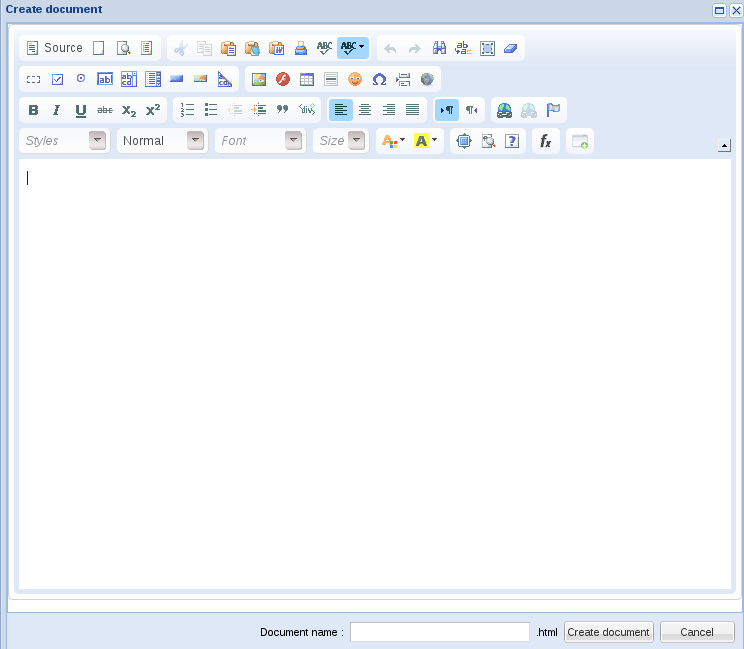
\includegraphics[scale=0.15]{Images/wysi.png} 
\end{minipage}& 
\\
\hline
\end{tabular}
\newline

\textbf{\underline {Create a document}} \\
\newline
\begin{tabular}{|m{3.7cm}|m{2.3cm}|m{4cm}|m{2.1cm}|}
\hline
\textbf{Name of the stage} & \textbf{Description}
 & \textbf{Expected result} & \textbf{Comments} \\
\hline
\begin{enumerate}
	\item Fill a description of a document

	\item Choose a name : test

	\item Select create document 
\end{enumerate}&
Display of the new document in the list : test.html & 
\begin{minipage}{0.7\textwidth}
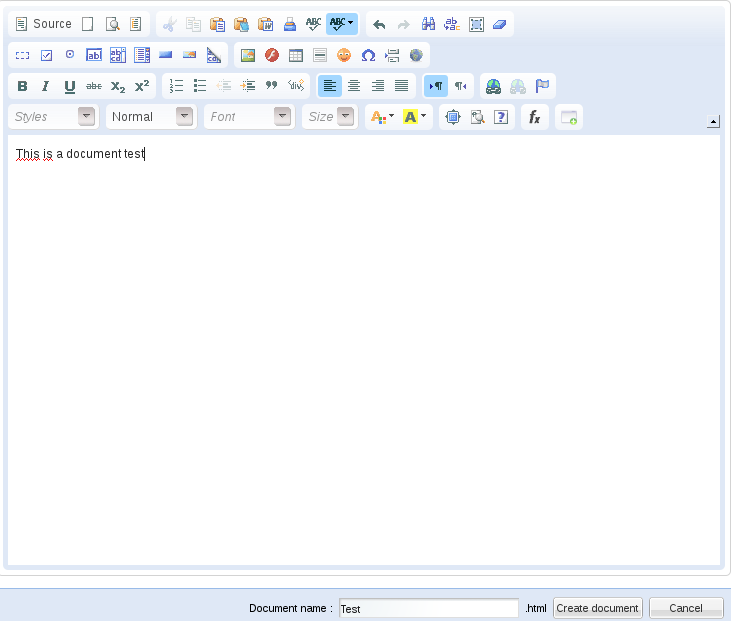
\includegraphics[scale=0.15]{Images/document.png} 
\end{minipage}& 
\\
\hline
\end{tabular}
\\
\newline

In the report, I created one section for each service. Then I accompanied 
each functionality with a formal description of the actions to perform, 
the eventual input data and their expected output. In the comments column, I wrote when the
functionality didn't work well or had a strange or not convenient beahaviour accoding to me. But then, 
if the comments was some kind of bugs or evolutions, I used Redmine to report them.  
My descriptions have to be as high level as possible in order to be understable for the customers. 

As a result of my work, the company had a useful document. It is now used to do regression
testing as I will explain in the next part. And it could be used to do automated tests later,
 all the scenarios to test are already written. And of course it would be given to the customers.
It is quite easy to evaluate the quality of the document, it has to be easy to read for
the regression tests that will consist in following all the steps detailed into it.\\


\subsection{Regression testing}
It is a kind of software testing that consists to uncover new softwares bugs
or regression. These tests are done after each change such as bugs fixing or new
 configurations settings made in the production instance. 
 Indeed, we can manage to fix a bug but 
meanwhile a new bug can appear. So regression testing aim to discover these
kind of new bugs, it helps to determine whether a change in one part of the
 software affects other parts of the software. 
 
 The tests I have done are called black box testing because I didn't know anything yet about
 the interior workings of the application, about the source code. The main advandage of this 
 testing method is that it clearly separates user's perspective from the developer's
 perspective. My role was to have a beahaviour as similar as possible to the one of 
 the future users.\\

The following is an example of test I had to do, which one lead to a bug I have found : 
On the school bag service when we clicked on the new Folder button, then on the close button. 
Then we couldn't click again on the new Folder button. The button was still displayed
 but when we clicked on it nothing would happen. I created a new Redmine issue to 
 report this bug.\\

Each time the team published changement in the production instance, I had to do some
regression testing. In order to do these tests, I used the technical report that I wrote
before. I ran set of test-cases by folowing the steps discribed in the document. 
For each test, I compare the results obtained with the expected results. 
If there is a correct match for the test, no new bugs had appeared for this functionality.
 If not, I reported the bug. 
 
 To report what I noticed during a specific test, I used Redmine and created an issue.
 In case of a correct match it can happen that the functionality tested is less convenient
 for the users than before. In this case I had to create an other kind of issue in Redmine,
 an evolution issue. These issues are usually less urgent to do. 
In each issues (bugs and evolutions), I described with precision what I detected. 
It is very  important to know in which environment the bug have been found such as 
Windows or Debian, Firefox, Google chrome or Internet Explorer as well as 
all the stages needed to reproduce the bug.  \\ 

Here is an example of a creation of Redmine issue : \\ 

\fbox{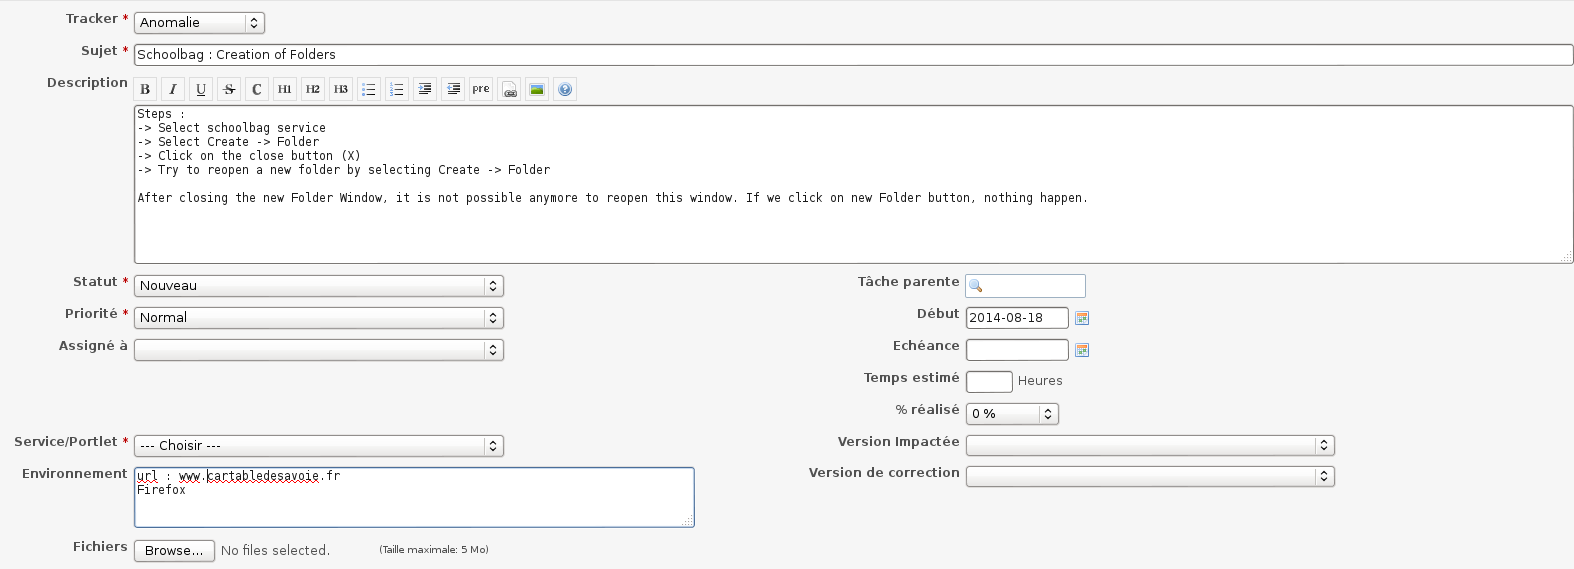
\includegraphics[scale=0.25]{Images/issue.png}} \\

All the redmine issues was then assigned to one member of the team developers and fix by
him. I will talk about this in the part called Bugfix. 


\newpage

\subsection{JMeter and some tools}
Part about JConsole and JMeter (if enough space)



